\section{\nn{} Runtime Energy Profiling} \label{sec:method1}

\nn{}'s runtime energy profiling method efficiently profiles the maximum drop of supply voltage that a task can cause, i.e. the aforementioned $\Delta \symb{V}{task}$. 
Unlike the previous disconnecting-supply method, \nn{}'s performs energy profiling with the supply connected, so as to reserve energy input during profiling.
Thus, $\Delta \symb{V}{task}$ cannot be measured simply by two voltage measurements at the beginning and the end of a task because the supply keeps charging the system during execution. 
Instead, \nn{} analyzes the supply current in the charge cycle, and uses it to derive $\Delta \symb{V}{task}$ in the discharge cycle. 
% Thus, this profiling method is more suitable for power supplies that change slowly, e.g. PV cells, so that input current does not change significantly in a charge-discharge cycle. 
% We will illustrate the mathematical reasoning of this method first, and then discuss possible imperfections in implementation. 

\nn{}'s runtime energy profiling method assumes an intermittent system is able to measure the supply voltage and to record time when asleep and active. 
The two functions can be achieved with efficient on-chip ADCs and timers on common off-the-shelf MCUs, e.g. MSP430FR series (an example platform used in intermittent computing literature). 

% (may goes to Method 2) 
% \item Ability to monitor the supply voltage and signal the MCU to wake up or sleep when a high or low threshold is hit. 
% Intermittent systems are also equipped with voltage monitoring function to determine when to wake up or sleep, which may be achieved by a voltage comparator~\cite{kang2018homerun, balsamo2016hibernus++}, an energy management unit~\cite{gomez2016dynamic, maeng2019supporting}, or a constant ADC polling. 

% Atomicity: no preemption during the task. 

\subsection{Principles}

To focus on the profiling rationale in the following illustration, we temporarily assume the mean supply current in a charge cycle remains the same in the next discharge cycle, both denoted as $\symb{I}{in}$. 
We will discuss the effect of volatile supply current shortly. 
We also omit the overhead of ADC voltage reading here. 

\begin{figure}[!t]
    \centering
    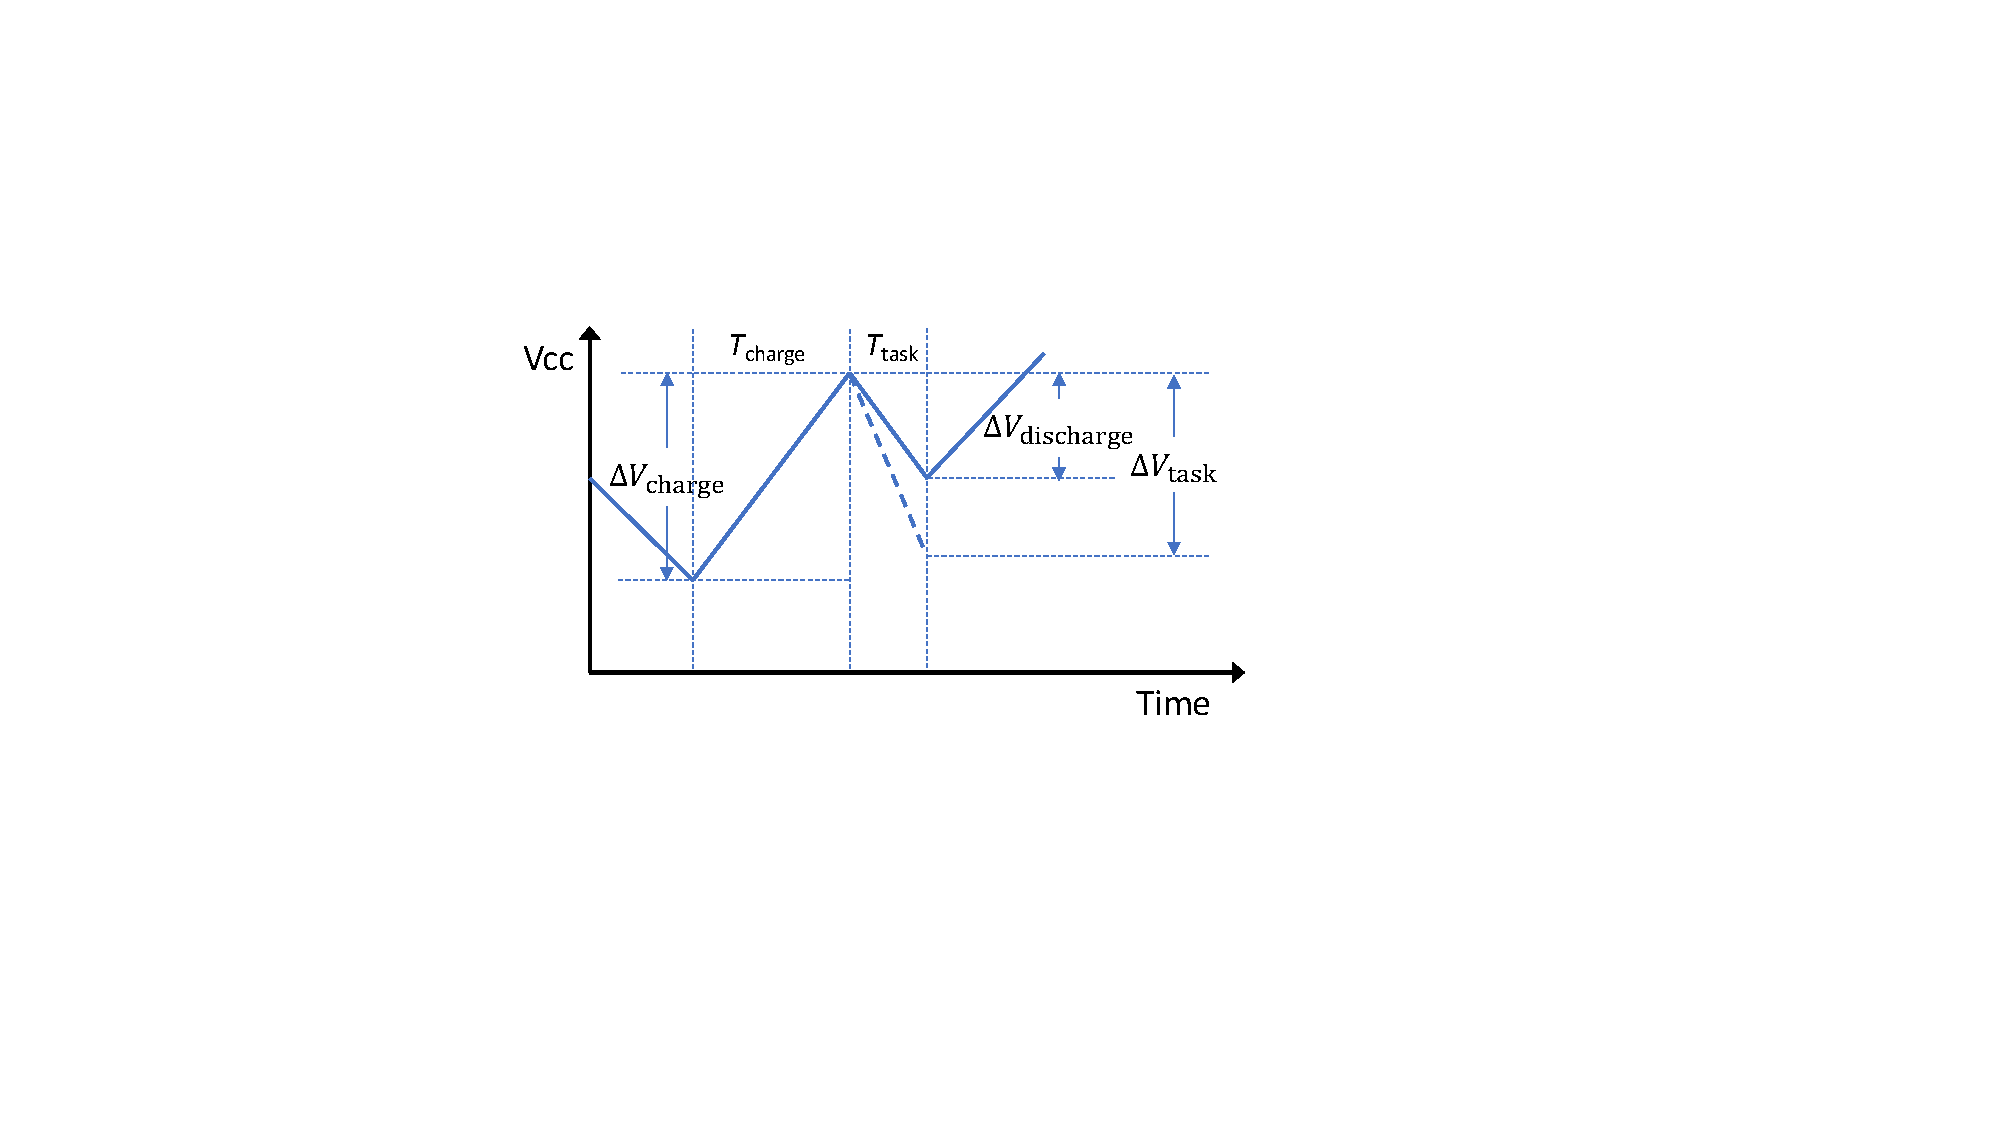
\includegraphics[width=0.8\columnwidth]{ch5_optic/figures/temp.pdf}
    \caption{An illustrative supply voltage trace for explaining \nn{}'s runtime energy profiling method. (To be replaced with a more 'academic' look) }
    \label{fig:math}
\end{figure}

\begin{table}[!t]
    \renewcommand{\arraystretch}{1.2}
    \centering
    \caption{Definitions of Mathematical Symbols}
    \label{tab:symbols}
    \begin{tabular}{|c|c|}
    \hline
    \textbf{Symbol} & \textbf{Definition} \\
    \hline
    $\Delta \symb{V}{task}$ & Maximum voltage decrease of a task \\
    $\Delta \symb{V}{charge}$ & Voltage increase of a charge cycle \\
    $\Delta \symb{V}{discharge}$ & Voltage decrease of a discharge cycle \\
    $C$ & System energy storage capacitance \\
    $\symb{I}{in}$ & Input current from energy harvester \\
    $\symb{I}{sleep}$ & System sleep current draw \\
    $\symb{I}{task}$ & System execution current draw during a task \\
    $\symb{T}{charge}$ & Time length of a charge cycle  \\
    $\symb{T}{task}$ & Time length of a task execution cycle  \\
    \hline
    \end{tabular}
\end{table}

We show an illustrative trace of supply voltage across a charge-discharge cycle in Figure~\ref{fig:math} with the symbols listed in Table~\ref{tab:symbols}. 

The system charge increase in the charging cycle can be described as
\begin{equation}
    \Delta \symb{V}{charge} C = (\symb{I}{in} - \symb{I}{sleep}) \symb{T}{charge}
    \label{eq:vcharge} 
\end{equation}
where $\symb{I}{sleep}$ is the current draw of the whole system when it sleeps and waits for energy refilling, including the current consumption for voltage monitoring, time recording, and other quiescent or leakage current.  

The system charge reduction in the discharging cycle can be described as
\begin{equation}
    \Delta \symb{V}{discharge} C = (\symb{I}{task} - \symb{I}{in}) \symb{T}{task}
    \label{eq:vdischarge} 
\end{equation}
where $\symb{I}{task}$ consists of the current draw of the main workload, voltage monitoring, time recording, and other quiescent or leakage current. 

The actual charge consumption of a task comes from the consumer part in (\ref{eq:vdischarge}), which is
\begin{equation}
    \Delta \symb{V}{task} C = \symb{I}{task} \symb{T}{task}
    \label{eq:vtaskc} 
\end{equation}

Hence, combining and rearranging (\ref{eq:vcharge}), (\ref{eq:vdischarge}), and (\ref{eq:vtaskc}), we can get the expression of $\Delta \symb{V}{task}$ as
\begin{equation}
    \Delta \symb{V}{task} = \Delta \symb{V}{discharge} + \Delta \symb{V}{charge} \frac{\symb{T}{task}}{\symb{T}{charge}} + \frac{\symb{I}{sleep}\symb{T}{task}}{C}
    \label{eq:vtask} 
\end{equation}

$\Delta \symb{V}{task}$ is the actual voltage drop that a task can cause, and directly determines the voltage threshold a system should set for the task to safely complete.
In (\ref{eq:vtask}), $\Delta \symb{V}{charge}$, $\Delta \symb{V}{discharge}$, $\symb{T}{task}$, and $\symb{T}{charge}$ are all perceivable values.
$\Delta \symb{V}{charge}$ and $\Delta \symb{V}{discharge}$ can be measured by three voltage readings at the transition points of charge and discharge cycles.  
$\symb{T}{task}$ and $\symb{T}{charge}$ can be measured with a on-chip timer. 

$\frac{\symb{I}{sleep}\symb{T}{task}}{C}$ is a theoretical profiling error of this approach.
If it is negligible or compensable, $\Delta \symb{V}{task}$ can be derived at runtime with all perceivable values. 

% \subsection{Realistic Considerations}

% There are some practical concerns that may affect the accuracy or efficiency. 

\subsection{Minimizing and Compensating Theoretical Profiling Error}

As the profiling method ignores the last term $\frac{\symb{I}{sleep}\symb{T}{task}}{C}$ in (\ref{eq:vtask}), the profiled value can be theoretically smaller than the actual one.
However, the empirical values of $\symb{I}{sleep}$, $\symb{T}{task}$, and $C$ in typical intermittent systems indicate that this error is relatively small. 
The system sleep current $\symb{I}{sleep}$ is a key property that is minimized in intermittent systems, and can be down to even sub-\SI{}{\micro\ampere} with modern low power techniques. 
The system capacitance $C$ is typically in \SI{}{\micro\farad} level in intermittent systems. 
The execution time of a task $\symb{T}{task}$ is typically a few or tens of \SI{}{\milli\second} as the energy buffering capacitor cannot afford a long, energy-hungry task. 
Hence, $\frac{\symb{I}{sleep}\symb{T}{task}}{C}$ should be typically under \SI{10}{\milli\volt}. 
This is insignificant compared to the voltage drop of a task (potentially hundreds of \SI{}{\milli\volt}), and can be easily or intrinsically compensated by margins in implementation.
For example, a voltage comparator may not have such resolution and precision, and thus may over-provision a small energy budget that compensate this error. 
% Also, the accuracy of voltage reading can also be 
Manually adding a small software offset to the profiling results can also overcome this error. 
Therefore, this theoretical profiling error is typically insignificant in implementation and easily compensated. 

% \todo{Refs for these rough numbers. Make a table for this?}
% Comment: And it's potentially possible to calibrate this error using the disconnecting supply method?}
    
\subsection{Effect of Volatile Supply Current}

The profiling method uses the average current input in the charge cycle as the current input in the next discharge cycle to derive the actual charge consumption. 
% This indicates the method would be more suitable for a current supply that does not usually change significantly across a charge-discharge cycle.
A charge-discharge cycle can be typically from tens to hundreds of \SI{}{\milli\second}, considering the capacitor size and the supply power in intermittent systems.
From our practical observation on some types of energy harvesters (e.g. PV cells), \nn{}'s profiling method performs stably (results presented in Section~\ref{sec:experiment}) as the supply current pattern complies with the assumption on supply current. 
However, we still anticipate there can be more volatile energy sources and analyze the consequent effect. 

% In intermittent systems, the energy buffering capacitor is typically small, e.g. tens of \SI{}{\micro\farad}, hence making the charge-discharge cycle short, e.g. tens to hundreds of \SI{}{\milli\second}. 

% Here, using this profiling result. 
% However, as $\symb{I}{in\_discharge}$ is increasing, the task can usually finish with the additional energy. 
We denote the the mean current in charge and discharge cycles as $\symb{I}{in\_charge}$ and $\symb{I}{in\_discharge}$ respectively. 
When $\symb{I}{in\_charge} > \symb{I}{in\_discharge}$, the system over-profiles $\Delta \symb{V}{task}$ by $(\symb{I}{in\_charge} - \symb{I}{in\_discharge}) \symb{T}{task} / C$ higher. 
When $\symb{I}{in\_charge} < \symb{I}{in\_discharge}$, the system under-profiles $\Delta \symb{V}{task}$ by $(\symb{I}{in\_discharge} - \symb{I}{in\_charge}) \symb{T}{task} / C$ lower. 
While the over-profiled energy budget should be safe, the under-profiled energy budget could be inadequate, making the following task failed. 
An unfortunate case is when the system first under-profiles a task with a rapidly increasing supply current, and then executes the task again using the newly profiled budget while no further energy is harvested during the execution. 
This can lead to a task failure, where the system needs other approaches in intermittent systems to maintain atomic progress, e.g. disabling checkpoints during atomic sections.

As discussed, \nn{}'s profiling method is suitable for energy sources that are not liable to change significantly across a charge-discharge cycle. 
If the energy source is too volatile to obtain reliable profiling results, a disconnecting-supply profiling method could be adopted as a workaround. 
% The over- or under-profiled value can be corrected when $\symb{I}{in\_charge}$ and $\symb{I}{in\_discharge}$ match again.

% \subsection{Discussion}

% The profiling method is intended to profile the latest energy consumption of a task with high energy efficiency, but not to guarantee the completion of the following tasks as they may have different consumption and the profiling result using this method could be less than the actual one. 

% threshold adaptation (e.g. increment after failure), for helping the Vth to restore quicker